\documentclass[a4paper,11pt,twoside]{article}
%\documentclass[a4paper,11pt,twoside,se]{article}

\usepackage{UmUStudentReport}
\usepackage{verbatim}   % Multi-line comments using \begin{comment}
\usepackage{courier}    % Nicer fonts are used. (not necessary)
\usepackage{pslatex}    % Also nicer fonts. (not necessary)
\usepackage[pdftex]{graphicx}   % allows including pdf figures
\usepackage{listings}
%\usepackage{lmodern}   % Optional fonts. (not necessary)
%\usepackage{tabularx}
%\usepackage{microtype} % Provides some typographic improvements over default settings
%\usepackage{placeins}  % For aligning images with \FloatBarrier
%\usepackage{booktabs}  % For nice-looking tables
%\usepackage{titlesec}  % More granular control of sections.

% DOCUMENT INFO
% =============
\department{Institution för Datavetenskap \\
Rapport obligatorisk uppgift}
\coursename{DV1: Datavetenskapens byggstenar 7.5 p}
\coursecode{DV160HT15}
\title{OU3 Tables}
\author{Lorenz Gerber  ({\tt{dv15lgr@cs.umu.se}})}
\date{2015-12-17}
%\revisiondate{2015-09-15}
\instructor{Lena Kallin Westin, Johan Eliasson, Emil Marklund, Lina Ögren}


% DOCUMENT SETTINGS
% =================
\bibliographystyle{plain}
%\bibliographystyle{ieee}
\pagestyle{fancy}
\raggedbottom
\setcounter{secnumdepth}{2}
\setcounter{tocdepth}{2}
%\graphicspath{{images/}}   %Path for images

% DEFINES
% =======
%\newcommand{\mycommand}{<latex code>}

% DOCUMENT
% ========
\begin{document}
\lstset{language=C}
\maketitle

\tableofcontents
\newpage

\section{Introduction} 
The aim with this laboration was to understand and a set of given 
composite data types and then built on those implement two new ones.
Test code for correctness and speed was given. The given datatypes
were directed \emph{list}, \emph{array}, and a \emph{table}, implemented using the 
aforementioned directed list. The used programming language was \emph{C}. 
The datatypes to be implemented were table using a \emph{move-to-front 
list} and \emph{table} using \emph{array}.

The implementation of the datatype \emph{table} is according to the 
defintion in the coursebook \cite[pp. 117 -- 132]{janlert2000}. In Brief:
a \emph{table} is a finite mapping of arguments to values. The textbook states 
a dictionary as a model where the lookup words are the arguments and the
textual explanations the values. The datatype \emph{table} however, does not 
need to be ordered by definition.

The operations found in the interface of a table are \emph{empty}, to create
an new empty \emph{table}, \emph{insert} to put new argument/value pair into an 
exisiting \emph{table}, \emph{isEmpty} to check whether an existing \emph{table} has any
content, \emph{lookup} to access the value associated to a potentially available
argument in an existing table and \emph{remove} to discard a potentially
existing argument/value pair from an existing table.  

The assigment included also testing and benchmarking of both the given and
the requested table implementations. The benchmarking was ment to
allow discussing the different implementations from a number of different
aspects such as lookup speed of existing and non-existing arguments, insertion
and removal speed as well as skewed or biased lookup. As a starting point,
a number of mandatory questions and discussion topics were given in the
lab instructions.  

\begin{figure}[H]
\centering
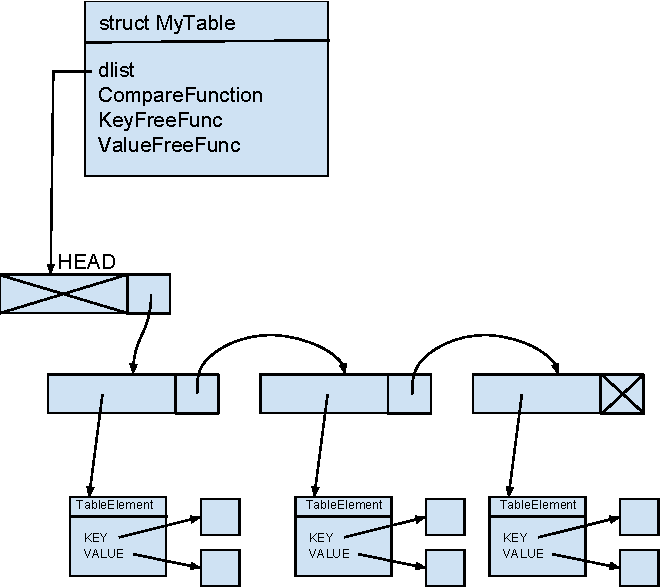
\includegraphics[width=0.7\textwidth]{figures/dlisttable.pdf}
\caption{\textit{Construction of the datatype dlist table and
    move-to-front list table.}}
\label{fig:dlisttable}
\end{figure}


\section{Material and Methods}
The description of the datatype \emph{table} in the introduction applies to
the actual implementations which will be described below. A small
difference is that the coursebook \cite{janlert2000}, uses the wording
\emph{argument} while the obtained implementation of a directed
list table uses the term \emph{key} in the code.  

\subsection{Directed List Table and Move-to-Front List Table}
The structure of a \emph{directed list table} and \emph{move to front list table} is
the same and can be seen in \textit{figure \ref{fig:dlisttable}}. The given
\emph{dlist} was constructed with a \emph{HEAD}, using physical and logical
position. The physical position is always one element before the logical. 
That means, when requesting content of the first list element, 
the pointer is directed to \emph{HEAD}. Then \emph{head->next}
will be used to access the content of the first cell. This setup is
needed in a single directional list mostly for the \emph{insert} operation:
The new element is inserted before the current element. If physical
and logical position would be the same, it would be needed to travers
the list again up to the position where the new element shall be inserted.

The special feature about the move-to-front list table is the lookup
operation: each time, an element is looked up, it is moved to the
front of the directed list. A schematic of this operation can be seen
in \textit{figure \ref{fig:movetofront}}. The arrows in black show the
initial situation and the red arrows new situation after moving the
looked up cell to the front. In \textit{figure \ref{fig:movetofront}},
the cell to be moved to the front is the one in the middle.

The request to remove a non-exisiting key result for both the given
\emph{directed list table} and the {move to front list table} in a traversal 
of the whole list, altough without any feedback. In case of duplicate
key values on an insertion, the old key/value pair is overwritten. In
more abstract terms, duplicates are handled at insertion time. 

\begin{figure}[H]
\centering
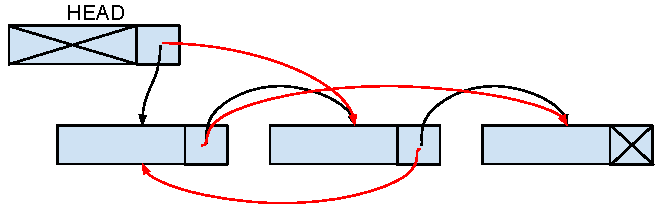
\includegraphics[width=0.5\textwidth]{figures/movetofront.pdf}
\caption{\textit{move to front operation in a directed list.}}
\label{fig:movetofront}
\end{figure}

\subsection{Array Table}
The structure of the {array table} can be seen in \textit{figure
  \ref{fig:arraytable}}. Instead of the \emph{directed list} it is now
an \emph{array} of \emph{void pointers}. The table is initialized to \emph{NULL
pointers}. On insertions, a \emph{void pointer} of the array field is then
set to point of the new table element. The current implementation
traverses the array from low to high until an array field with a \emph{NULL
pointer} or the same \emph{key} as the one to insert is found. On removal
of a key/value pair, the whole \emph{array} is traversed to discard eventual
duplicate \emph{key} entries. In more abstract terms, duplicates are handled
partly at insertion time and partly but definite at removal time. 
If a non-existing \emph{key} is given as argument to
the remove operation, the whole \emph{array} will be traversed. In the
current implementation no feedback is given whether a key was found
and removed or not.   

An important feature to mention is that by definition an array is a 
static datatype while a table is dynamic. This will be discussed in 
more detail. Also by definition, they index of an array is usually a 
natural number or integer which does not match with the definition of 
the argument/key in a table. A direct mapping from argument/key to 
array index is therefore in the most general case not possible. 


\begin{figure}[H]
\centering
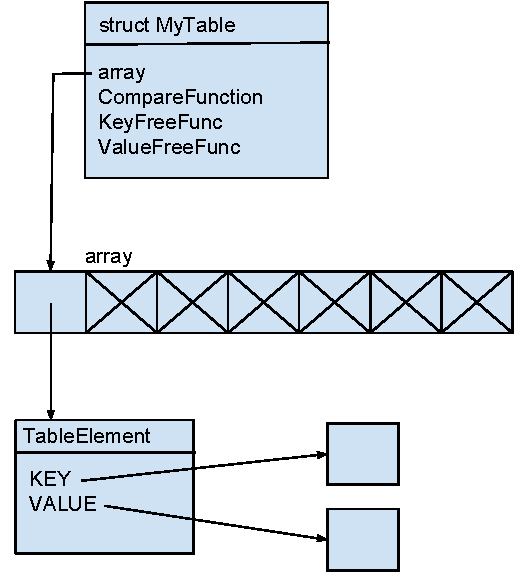
\includegraphics[width=0.5\textwidth]{figures/arraytable.pdf}
\caption{\textit{Construction of the array table data type.}}
\label{fig:arraytable}
\end{figure}

\subsection{Proposed changes to the interface}
Currently, the interface specification does not implement any 
return value for the operations \emph{remove},\emph{insert} and 
\emph{free}. For
those three, a boolean feedback whether the operation succeeded or not
could make sense. This would for example provide the information
whether a \emph{key} requested for removal was available in the table or
not. For the \emph{insert} operation, it could provide a signal in the
\emph{table array} implementation when the underlying array is full with
values. 


\section{Results}
\subsection{Correctness of datatype implementations}
To assess the correctness of the implemented datatypes a set of eight
tests was provided:

Correctness of the data types was assessed by eight
\begin{itemize}
\item {isEmtpy} on a new created table yields TRUE
\item insert a single element
\item lookup a single element
\item insert and lookup multiple elements with non identical keys
table
\item insert and lookup multiple elements with identical keys
\item remove a single element
\item remove elements with different keys
\item remove elements with the same key
\end{itemize}

The tests followed to a large extent the axiomatic table defintion given
in the course book \cite[p 122]{janlert2000}. All the implemented
tables fulfilled the test criteria.

\subsection{Performance tests}
The performance of the implemnted datatypes was assed by five
different tests that represent typical operations and use cases for
the datatype \emph{table}. 

\begin{itemize}
\item Insertion speed
\item random existing lookup speed
\item random non-existing lookup speed 
\item skewed lookup speed
\item remove speed  
\end{itemize}

All above mentioned tests took as parameter the number \textit {n} 
of operations to be run for each separate test. This allows to assess the
time-complexity when performing the test for a series of increasing
\textit{n}. The test data generation procedure was also provided and
was based on the C \emph{rand} function. To account for worst/best case
scenarios stemming from the random numbers, each test was run 10
times. Results below are presented as scatter plots (a) with
arithmetic means of ten runs for each \textit{n} operations case. 
The (b) plots show the relative standard deviation (RSD) for the 10
replicate runs in each \textit{n} operations point.  

To simplify the whole procedure, an additional block of code was added
to each test function which caused to append the test results to a text
file with the name \emph{benchmark.txt} (listing \ref{code:benchmark}).

\begin{lstlisting}[label=code:benchmark,caption=code block for writing
  benchmark data to file]
FILE *f = fopen(``benchmark.txt'', ``a'');
fprintf(f, ``%lu",end-start);
fprintf(f,"\t");
fclose(f);
\end{lstlisting}

The text files where then imported into the statistical programming language `R'
\cite{rlanguage}. Data aggregation, statistics and plotting was done
in the aforementioned language according to a separate protocol
(attachement).

The five first result figures (\textit{Figures \ref{fig:insertion} to
\ref{fig:remove}}) present data on a per test basis. The
\textit{(a)} plots show the average benchmark time for 7 datapoints 
(\textit{n = 250, 500, 1000, 2500, 5000, 7500, 10'000}). Each plot
contains three data series for the benchmarked datatypes.

The \textit{(b)} plots present the relative standard deviation (RSD)
of the experiments shown in \textit{(a)}. 

\textit{Figure \ref{fig:dlist} to \ref{fig:array}} show average test time and
RSD per data type for 3 selected benchmarks (\emph{Random Existing Lookup},
\emph{Random Non-Existing Lookup} and \emph{Skewed Lookup}). Those three figures
show now new data but allow more convenient intpretations compared to
the per test figures.

\begin{figure}[H] 
\centering 
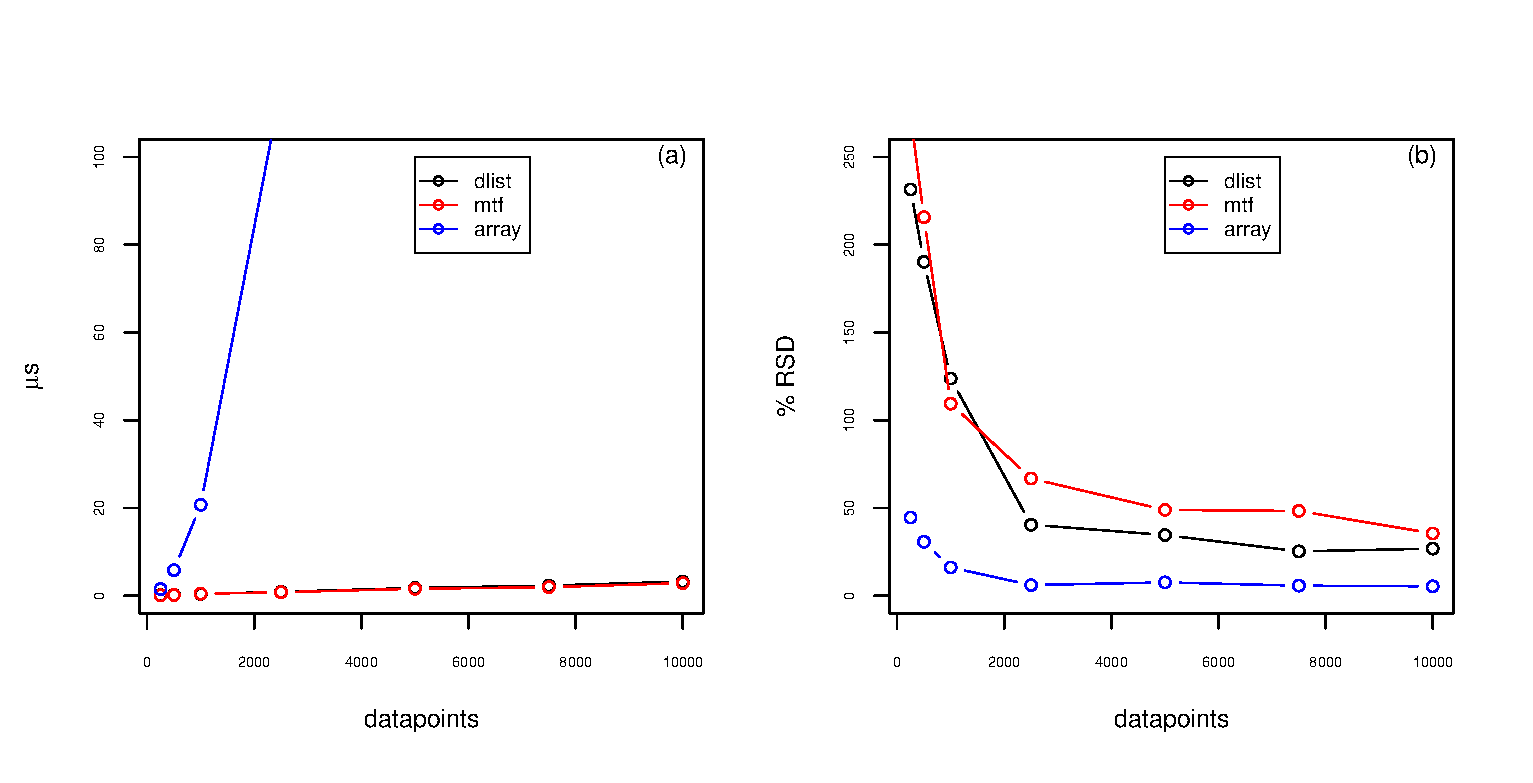
\includegraphics[width=\textwidth]{figures/fig1.eps}
\caption{\textit{Figure 1a, shows the element \textbf{`insertion'}
    times. Figure 1b shows the RSDs from the measurments in figure 1a. n=10.}}
\label{fig:insertion}
\end{figure}

\textit{Figure \ref{fig:insertion}} shows the results for the
\emph{insertion} benchmark. The speed for \emph{dlist} and \emph{mtf} datatype were
about the same while the \emph{array} implementation was much slower. It
should be noted that for all conducted tests on the \emph{array}
implementation, the size of the \emph{array} was always adapted to the
needed size. RSD's for the \emph{array} implementation were lower than for
the other two data types altough with a similar behaviour: High RSD's 
for small \textit{n's} and lower for high \textit{n's}. The curves
decreases quick at low towards higher \textit{n's} and becomes very
flat and stable after about 5000 \textit{n}.

\begin{figure}[H] 
\centering 
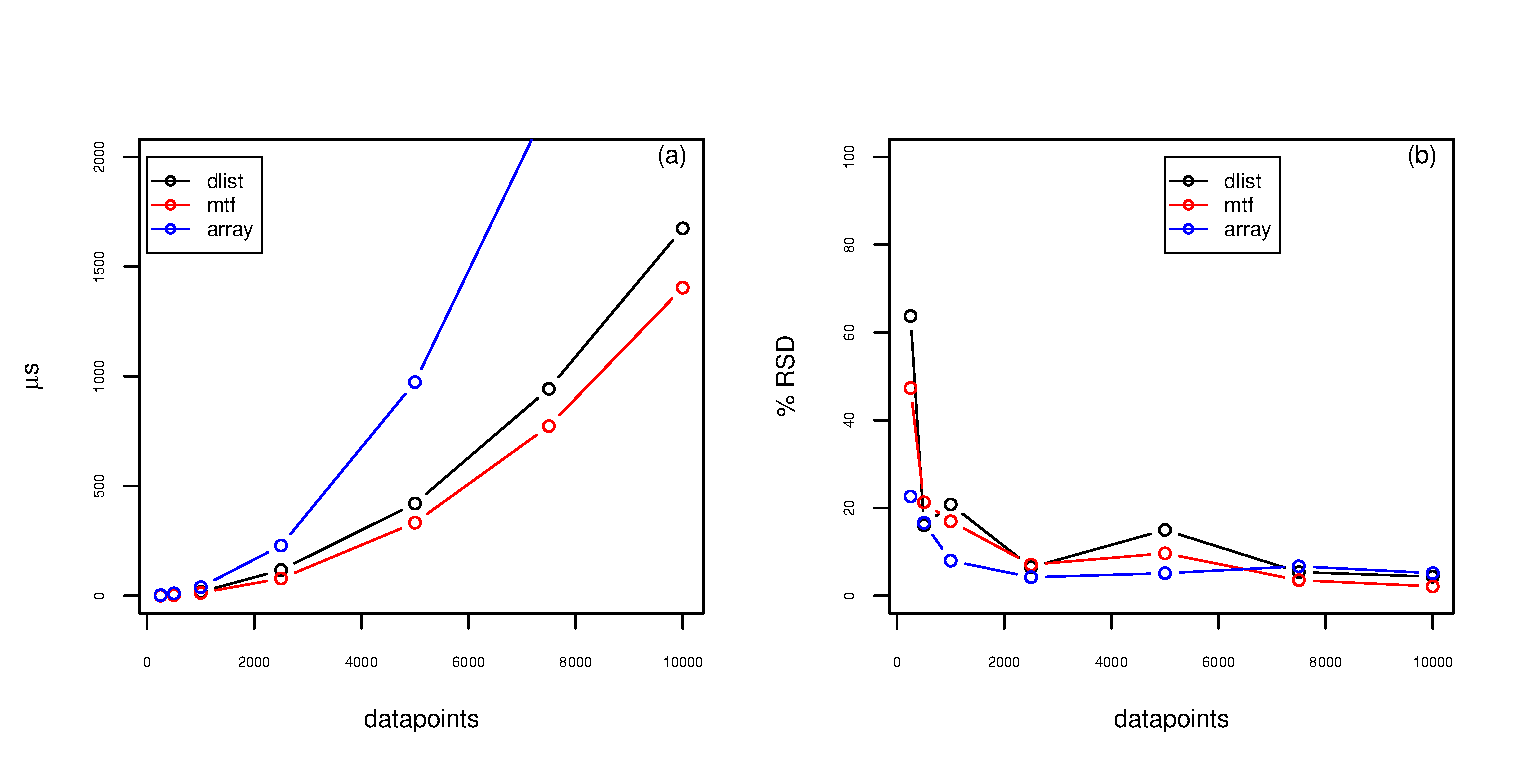
\includegraphics[width=\textwidth]{figures/fig2.eps}
\caption{\textit{Figure 2a, shows the times for the \textbf{`Random Existing
    Key Lookup'} benchmark. Figure 2b shows the RSD's from the measurments
in figure 2a. n=10.}}
\label{fig:randexlook}
\end{figure}

\textit{Figure \ref{fig:randexlook}} shows the results for the \emph{Random
Existing Key Lookup} test. \emph{dlist} and \emph{mtf} datatypes show smimilar
mean times while \emph{array} is again the slowest. The RSD's are very
similar for all benchmarked datatypes.

\begin{figure}[H] 
\centering 
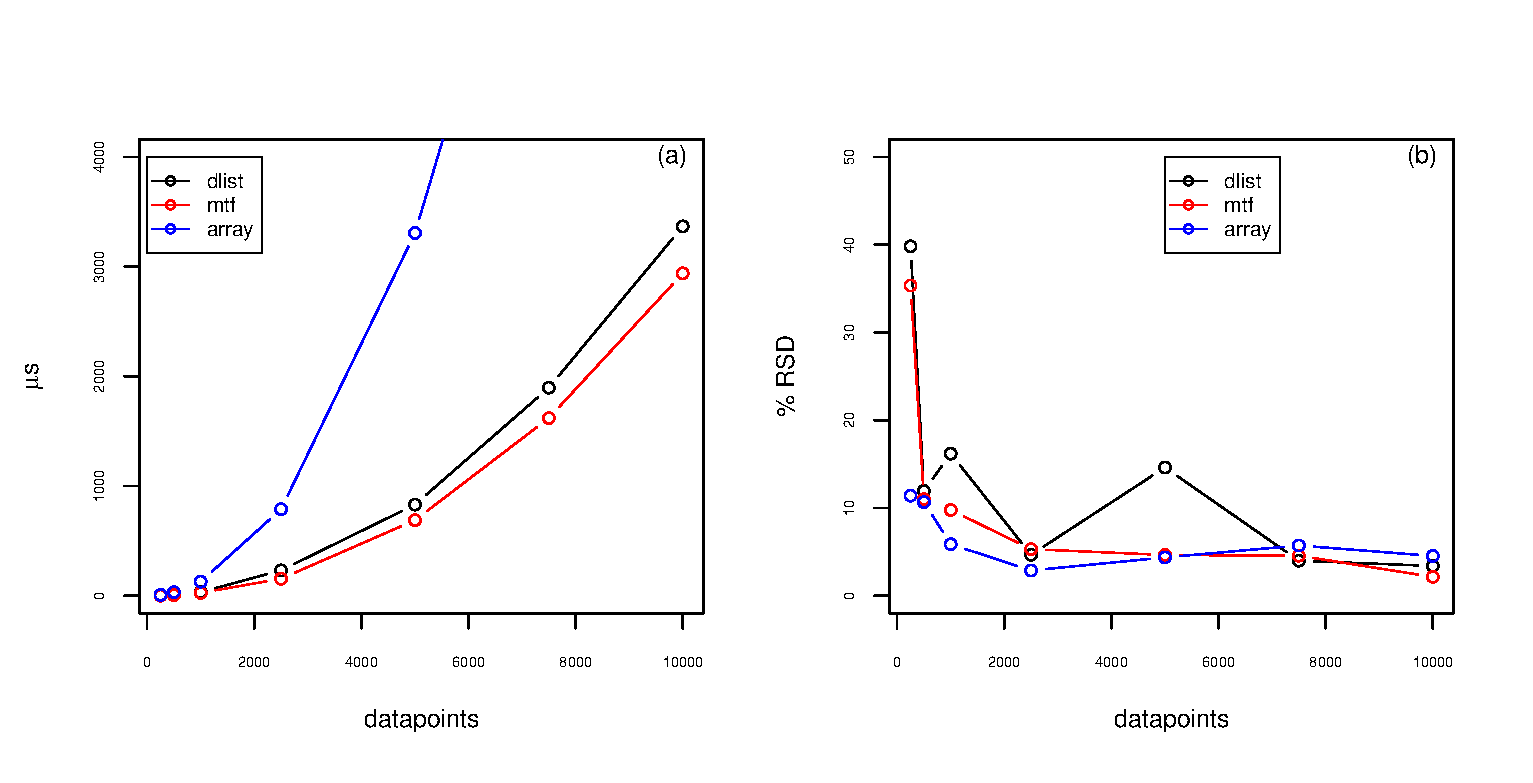
\includegraphics[width=\textwidth]{figures/fig3.eps}
\caption{\textit{Figure 3a, shows the times for the \textbf{`Random
      Non-Existing Key Lookup'} benchmark. Figure 3b shows the RSD's from
    the measurments in figure 3a. n=10.}}
\label{fig:randnonexlook}
\end{figure}

\textit{Figure \ref{fig:randnonexlook}} shows the results for the
\emph{Random Non-Existing Key Lookup} benchmark. The times are about double
compared to the \emph{Random Existing Key Lookup} test with the same
ranking where \emph{dlist} and \emph{mtf} are about the same and the \emph{array}
implementation is the slowest. The RSD's for \emph{mtf} and \emph{array}
datatype look similar as in the \emph{Random Existing Key Lookup} however
the \emph{dlist} resulted in a peculiar irregular curve shape for the
series of increasing \textit{n}. On closer inspection, a similar curve
shape, although less pronounced can be found for all RSD value series
of the \emph{dlist} datatype.

\begin{figure}[H] 
\centering 
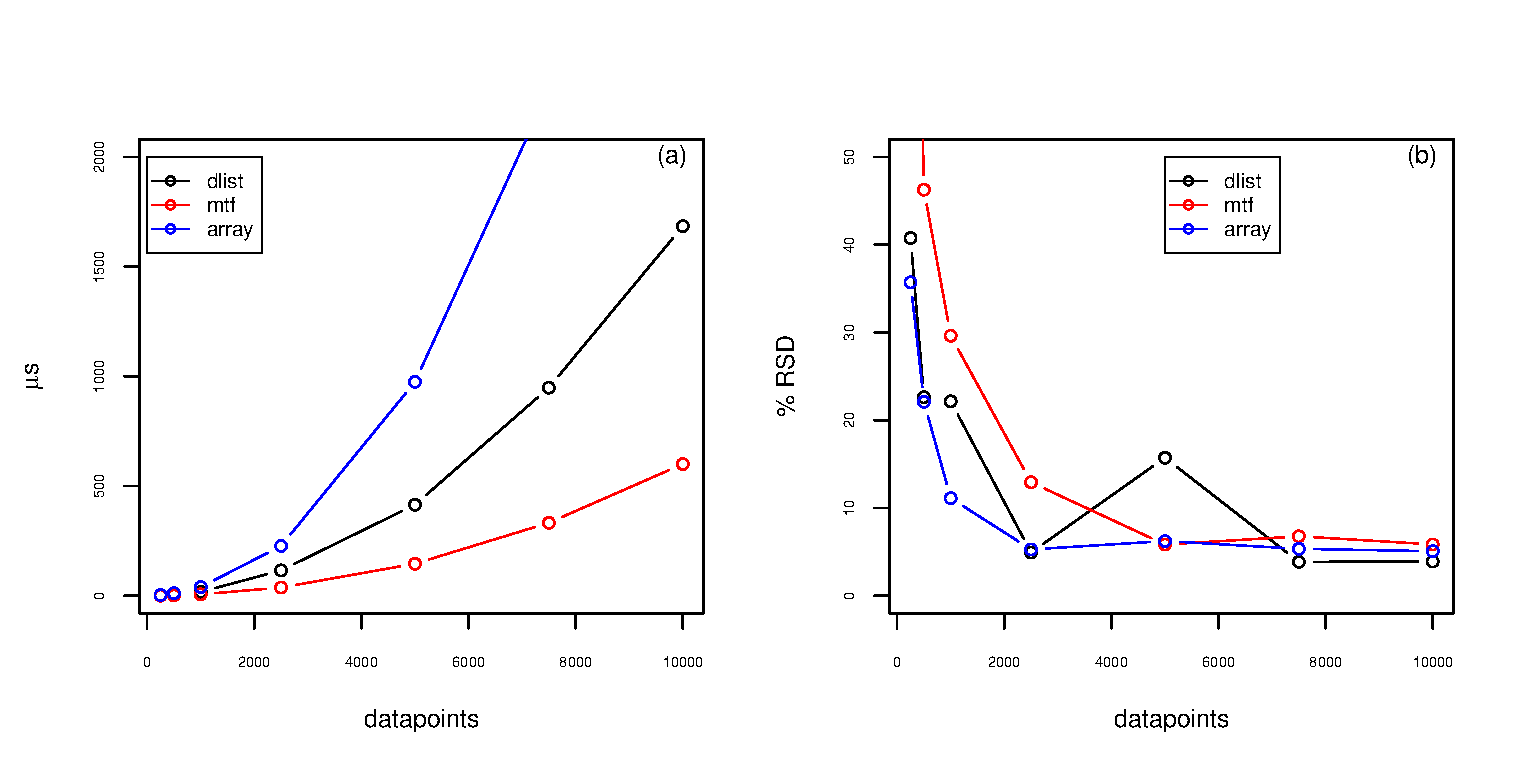
\includegraphics[width=\textwidth]{figures/fig4.eps}
\caption{\textit{Figure 4a, shows the times for the \textbf{`Skewed
      Lookup'} benchmark. Figure 4b shows the RSD's from the
    measurments in figure 4a. n=10.}}
\label{fig:skewed}
\end{figure}

\textit{Figure \ref{fig:skewed}} shows the results for the 'Skewed
Lookup' benchmark where the some values are looked up with a higher
frequency than random. Here the \emph{mtf} implementation is by far the
fastest followed by the \emph{dlist} and slowest again the \emph{array}
implementation. The RSD's are similar as for the two affore mentioned
benchmarks.


\begin{figure}[H] 
\centering 
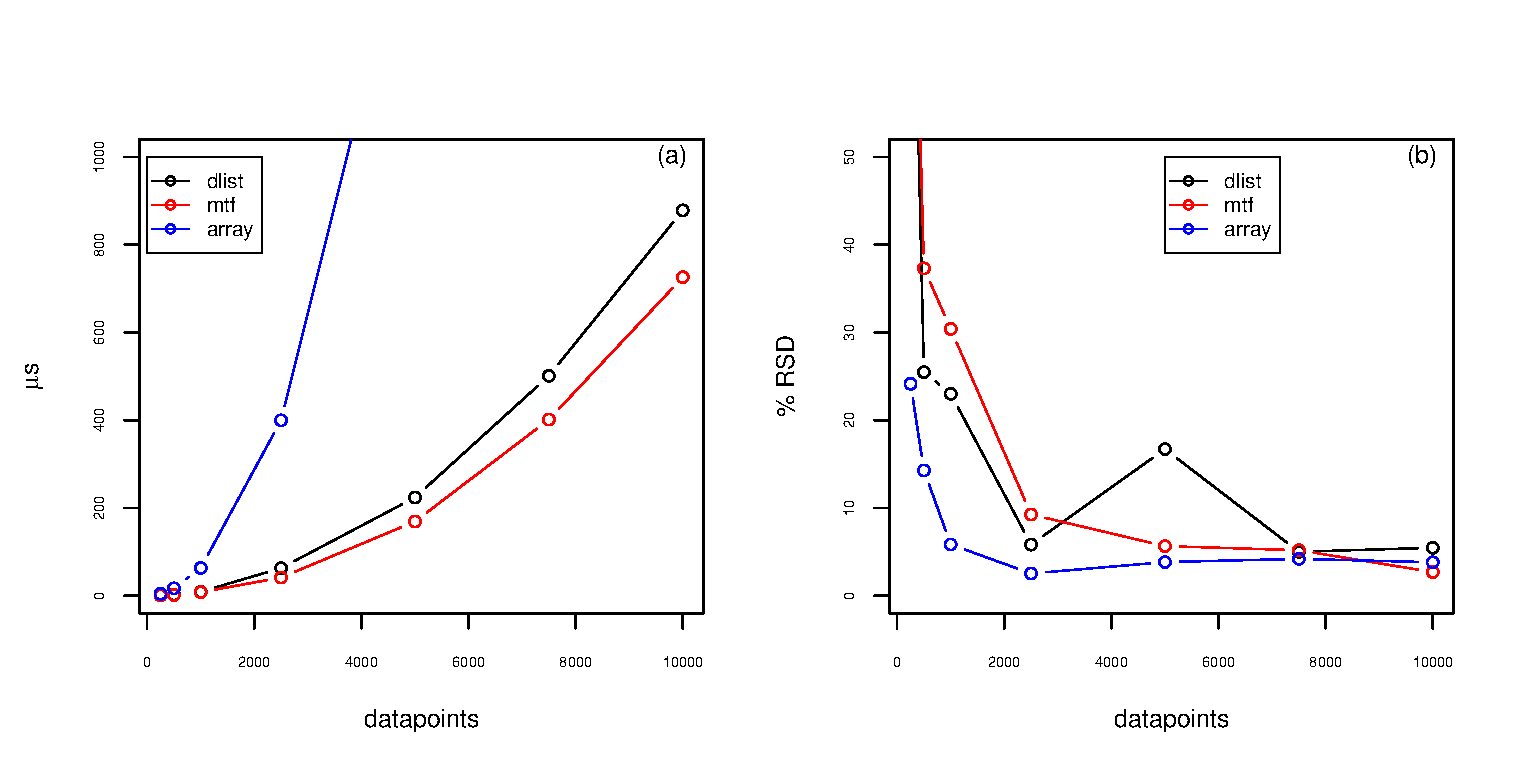
\includegraphics[width=\textwidth]{figures/fig5.eps}
\caption{\textit{Figure 5a, shows the times for the \textbf{`Removal'}
    benchmark. Figure 5b shows the RSD's from the measurments in figure 5a. n=10.}}
\label{fig:remove}
\end{figure}

\textit{Figure \ref{fig:remove}} shows the results for the \emph{Removal}
benchmark. The plot look similar like the \emph{Random Non-Existing Key
Lookup} however the times are a bit faster for all datatypes. The
RSD's are in the same range as for the other benchmarks (excpet the
insertion). 

\begin{figure}[H] 
\centering 
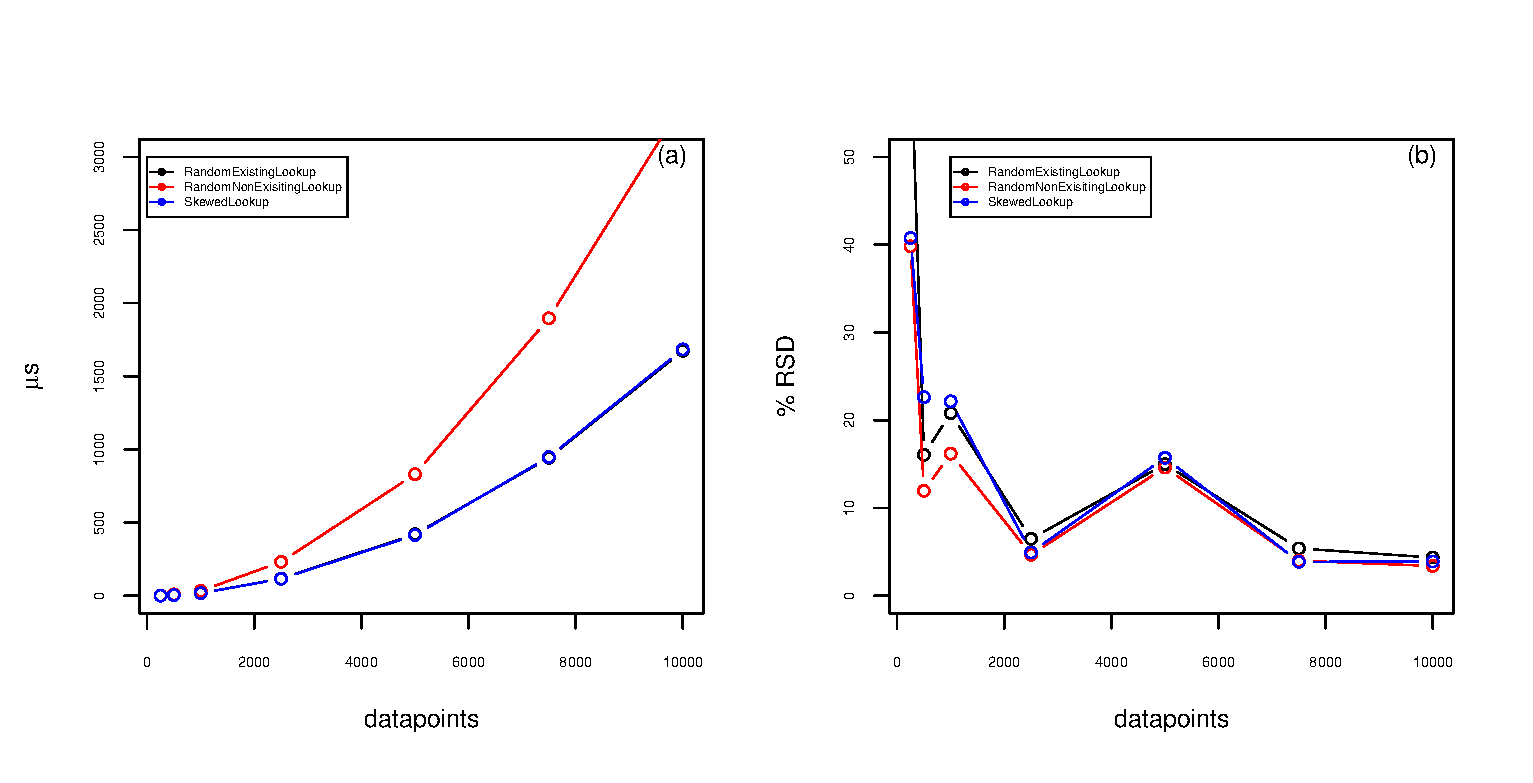
\includegraphics[width=\textwidth]{figures/fig6.eps}
\caption{\textit{Figure 6a, shows the times for the \textbf{`Random Existing
    Lookup'}, \textbf{`Random Non-Exisiting Lookup'} and
  \textbf{`Skewed Lookup'} benchmark of the datatype \textbf{`dlist'}. Figure 6b shows the RSD's from the measurments
in figure 6a. n=10.}}
\label{fig:dlist}
\end{figure}

\textit{Figure \ref{fig:dlist}} shows the results for the benchmarks
\emph{Random Existing Key Lookup}, \emph{Random Non-Existing Key Lookup} and
\emph{Skewed Lookup} for the datatype \emph{dlist}. \emph{Random Existing Key Lookup} and
\emph{Skewed lookup} are exactly equal fast while \emph{Random Non-Existing Key
Lookup} is a bit slower. Note the peculiar shape of the RSD data curves.

\begin{figure}[H] 
\centering 
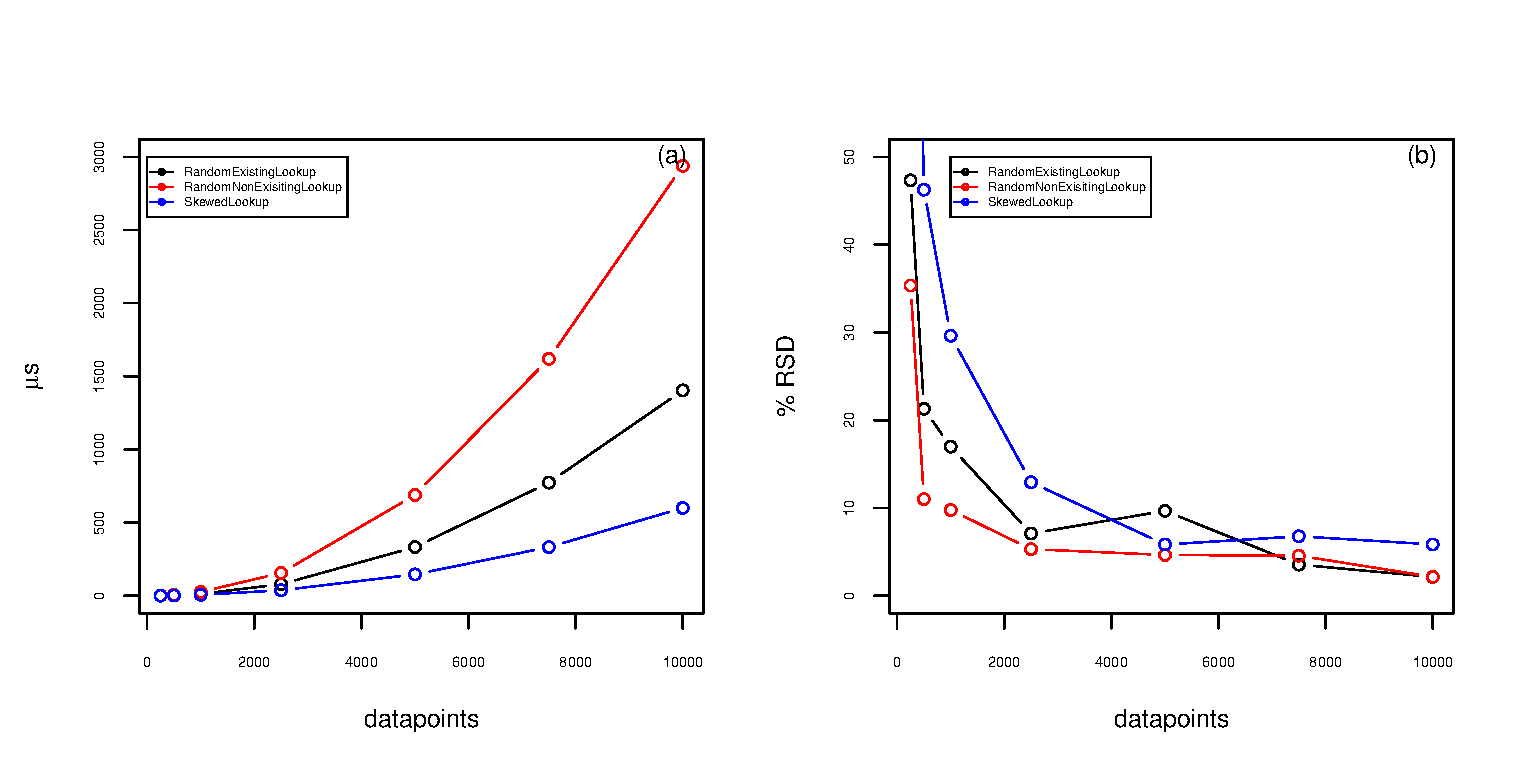
\includegraphics[width=\textwidth]{figures/fig7.eps}
\caption{\textit{Figure 7a, shows the times for the \textbf{`Random Existing
    Lookup'}, \textbf{`Random Non-Exisiting Lookup'} and
  \textbf{`Skewed Lookup'} benchmark of the datatype \textbf{`mtf'}. Figure 7b shows the RSD's from the measurments
in figure 7a. n=10.}}
\label{fig:mtf}
\end{figure}

\textit{Figure \ref{fig:mtf}} shows the results for the benchmarks
\emph{Random Existing Key Lookup}, \emph{Random Non-Existing Key Lookup} and
\emph{Skewed Lookup} for the datatype \emph{mtf}. \emph{Skewed lookup} here is by 
far the fastest followed by \emph{Random Existing Key Lookup} and 
\emph{Random Non-Existing Key Lookup}. RSD's are similar for the three
cases with the common pattern, high and quick decreasing for very low
\textit{n} while low and almost flat for higher \textit{n} values.

\begin{figure}[H] 
\centering 
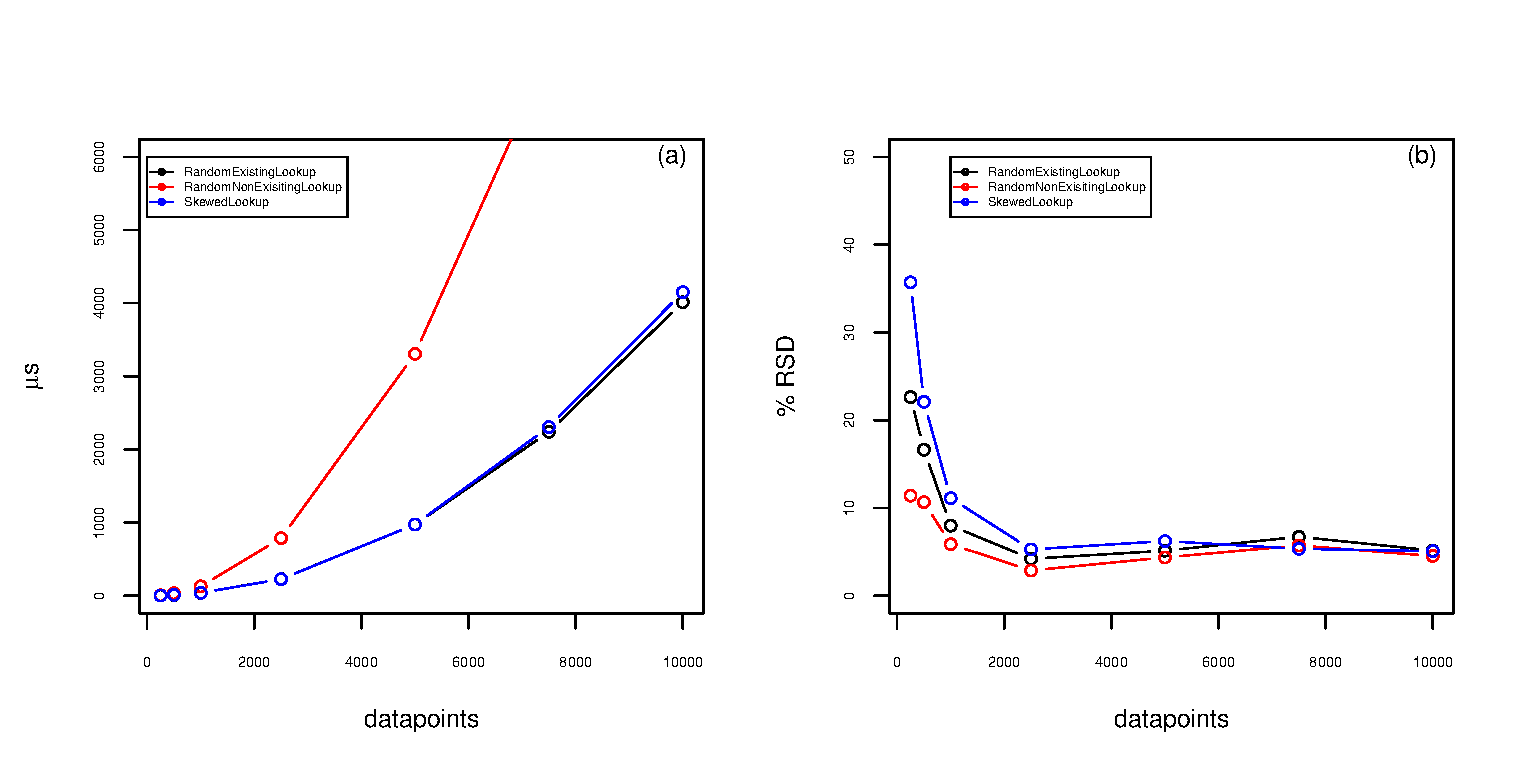
\includegraphics[width=\textwidth]{figures/fig8.eps}
\caption{\textit{Figure 8a, shows the times for the \textbf{`Random Existing
    Lookup'}, \textbf{`Random Non-Exisiting Lookup'} and
  \textbf{`Skewed Lookup'} benchmark of the datatype \textbf{`array'}. Figure 8b shows the RSD's from the measurments
in figure 8a. n=10.}}
\label{fig:array}
\end{figure}

\textit{Figure \ref{fig:array}} shows the results for the benchmarks
\emph{Random Existing Key Lookup}, \emph{Random Non-Existing Key Lookup} and
\emph{Skewed Lookup} for the datatype \emph{array}. \emph{Random Existing Key Lookup} and
\emph{Skewed lookup} are exactly equal fast while \emph{Random Non-Existing Key
Lookup} is a bit slower. The RSD's are very regular and stable among
the three test cases.


\section{Discussion}
Ranking according speed for the different datatypes was obvious. 
The slowest implementation in every aspect by far is
\emph{array} while \emph{dlist} and \emph{mtf} are about equal, except for the
\emph{Skewed Lookup} test where the \emph{mtf} implementation is fastest. 
The \emph{Move-to-Front} strategy seems to be tailored for this
situation. There should be quite a lot of real world
applications where the distribution of lookup keys is not randomly
distributed but rather skewed. A typical application could be webshops.
There performance improvements can be obtained by \emph{mtf} as there will
usually be a number of \emph{favourite} products accessed more often by 
customers than other products.

For operations where always or in the worst case a full
traversal of the data whole structure is needed, it is obvious that the
\emph{array} implementation is slowest. However it is not obvious to me with this
reasoning why the \emph{array} implementation is slower for \emph{insertion} and
\emph{removals}. It can be noted from the axis scale in \textit{figure
  \ref{fig:insertion}} and \textit{\ref{fig:remove}} that insertion is
still quite a bit faster than removal. While the time critical
operation in removal should be the time needed for a full traversal, 
this can not be the reason for slow performance on insertions. 
A hypothesis is that allocating a large amount of memory at once, 
as it is the case for \emph{array},  takes a longer time than allocating 
several times very short address ranges. 

An obvious disadvantage of the \emph{array} implementation is also the
static character which it forces onto the \emph{table}. A table is by 
defintion a dynamic datatype. When implementing the \emph{table} with an
\emph{array} this is then just valid for a limited operational envelope,
the size of the array. A small advantage of the \emph{array} implementation 
could be the very stable and well defined RSD's. They suggest that 
worst and best case are very similar for this implementation and as 
such the response times very predictable. However, whether this difference to the two
other implementations is really significant would have to be tested
statistically. One thing to note regarding the RSD's is the peculiar
pattern found for the \emph{dlist} datatype on a series of different
\textit{n} values. A simple statement describing this observed pattern
could be: The RSD for replicates at 5000 operations is higher than the
RSD at 2500 operations. This does not sound logica and at the moment, 
I don't have a reasonable explication for it, but the phenomena seems
to replicable as it occoured in all three benchmarks 
\textit{(Figure \ref{fig:dlist}(b))}.

While most of the presented results suggest that implementing a
\emph{table} by an \emph{array} is a bad choice, there are some
exceptions: For a table implementation where keys are exclusively 
natural numbers/integers that do not spread over a large value range, 
an \emph{array} should yield a very fast datatype. This comes from the fact
that for the expensive operations \emph{lookup}, \emph{insert} and \emph{remove} no
traversal is needed. It will be quick direct acces. Also no expensive
handling of duplicate values is needed in this case.  

\addcontentsline{toc}{section}{\refname}
\bibliography{references}

\end{document}
